\section{The Greenland ice sheet model}

% Is the model set up correctly, i.e., as per instructions and without coding errors? (10 points)
% Is the performance of the model sufficiently documented with figures and (quantified) analysis? At least one figure showing the ice thickness should be shown, and one section through the ice sheet. (5 points)
% Discuss if the model is producing accurate results. Why do you trust it? (5 points)

The GrIS is simulated using a two-dimensional ice flow model. Generally speaking, ice flow is driven by hydrostatic pressure exerting differential shear stress due to variations in glacier height. Glen's flow law, an empirical relation between strain rate and stress, allows to derive the vertically-integrated velocity
\begin{equation}\label{eq:meanu}
\mean{u} = -\frac{2}{5}A \left( \rho g \delta_x z \right)^3 h^4,	
\end{equation}
where \(A\) is the so-called flow parameter, \(\rho\) the ice density, \(g\) the gravitational acceleration, \(z\) the surface elevation, and \(h\) the ice thickness. 
\Cref{eq:meanu} can be extended to an ice flux \(F\), which in turn, combined with the surface mass balance  \(M\) (i.e., the net balance of accumulation and ablation) yields the change of ice thickness in time 
\begin{equation}\label{eq:flux}
	\delta_t h = -\nabla F + M = -\nabla (\mean{u}h) + M.
\end{equation}

\subsection{Benchmarking}

In order to initially verify the ice flow model, a benchmark simulation spanning \SI{10000}{\year} is performed. The spatial domain of this simulation (like all others) has a resolution of \SI{40}{\km}. It is run on flat bedrock, paired with an artificial surface mass balance (SMB). Inside a 10\(\times\)10 grid box the SMB is positive (\(M = \SI{2}{\m\per\year}\)), while outside this area \(M = \SI{-2}{\m\per\year}\) is applied. \Cref{fig:benchmark-map} indirectly illustrates the benchmark SMB in the upper-left subplot, since the growing ice thickness matches the area of positive SMB. On top, we observe that the expansion of the ice ultimately reaches an equilibrium in the shape of a circle with maximum ice thickness at its centre. 

\begin{figure}
	\centering
	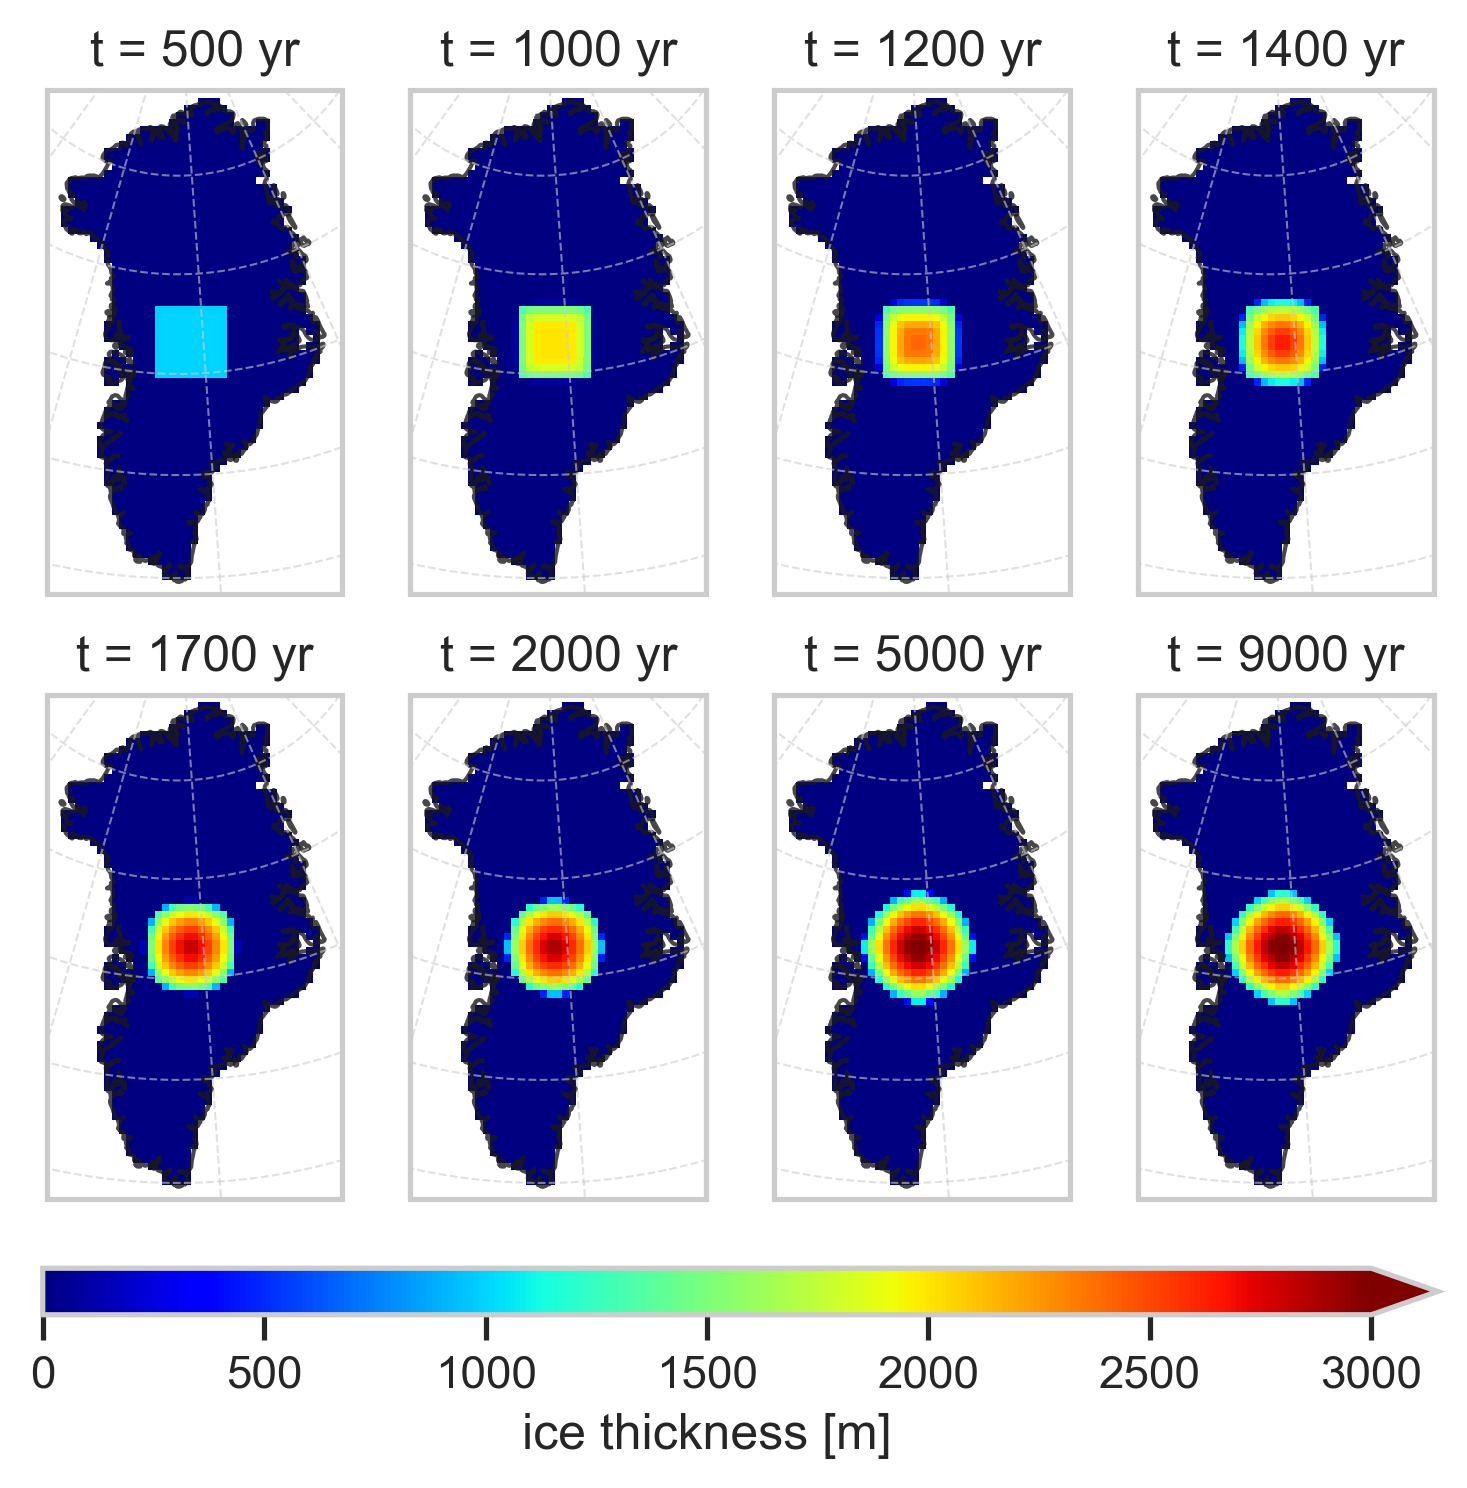
\includegraphics[width=0.7\linewidth]{../benchmark/figs/ice-map.png}
	\caption{Map of ice thickness at time steps \(t\) during the benchmark simulation}
	\label{fig:benchmark-map}
\end{figure}

\begin{figure}
	\centering
	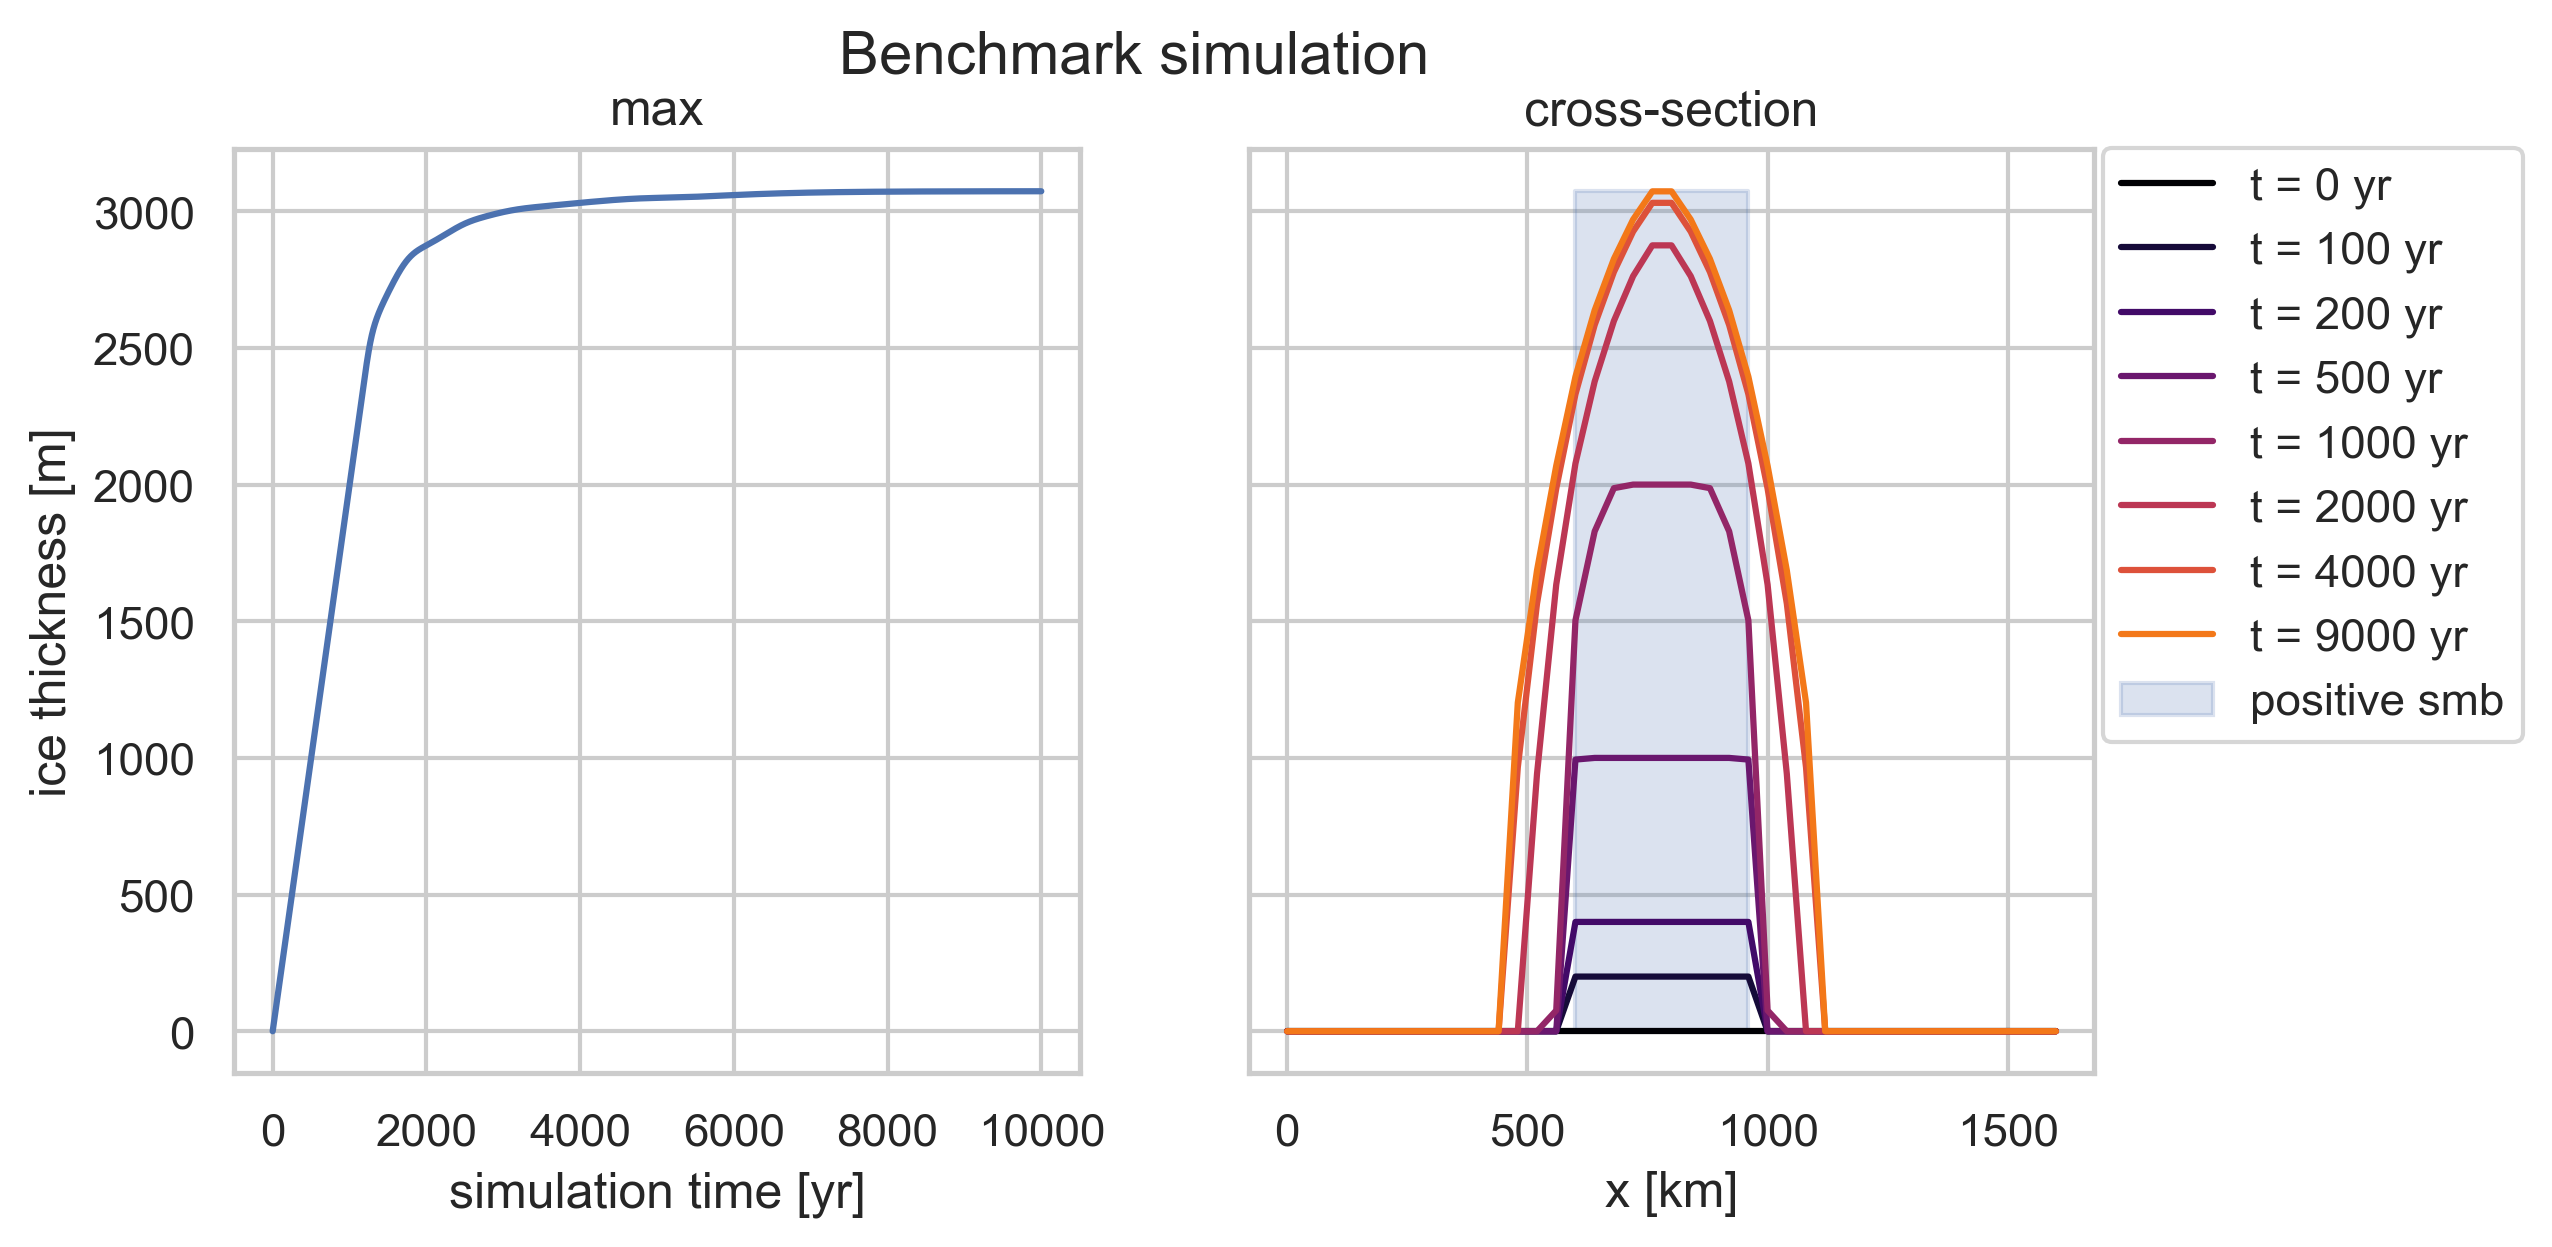
\includegraphics[width=\linewidth]{../benchmark/figs/cross-section.png}
	\caption{\textit{Left:} Maximum ice thickness throughout simulated years. \textit{Right:} West-east cross-section of ice thickness; the region of positive SMB is found in-between the dashed lines.}
	\label{fig:benchmark-cross-section}
\end{figure}

The equilibrium state is characterized by a maximum ice thickness of just over \SI{3000}{\m} after approximately \SI{4000}{\year} of simulation  (\cref{fig:benchmark-cross-section}). The ice flow becomes increasingly noticeable from \SI{1000}{\year} onwards, after an ice thickness of around \SI{2000}{\m} has been reached. From \(F \propto h^5\) in \cref{eq:flux} it is to be expected that a certain height has to be reached before considerable ice flow can occur. Qualitatively, the isotropic flow and shape of the ice sheet is comparable to the results of other students and the benchmark data agrees well with what has been mentioned in the (video) lectures.

\subsection{Surface mass balance}\label{sec:smb}

After benchmarking the simulation, the upcoming model runs feature a more realistic SMB. The annual melting \(\mathrm{M}\) of the ice sheet is derived from an artificial temperature field \(T\) using a positive degree day approach
\begin{equation}\label{eq:melt}
	\mathrm{M} = \beta \cdot \sum_{i=\mathrm{Jan\, 1}}^{\mathrm{Dec\, 31}} \max \left(T_{i},\SI{0}{\celsius}\right),
\end{equation}
while the accumulation \(\mathrm{A}\) is simplified to all precipitation \(P\) at temperatures below the freezing point 
\begin{equation}\label{eq:acc}
	\text{A} = \sum_{i=\mathrm{Jan\, 1}}^{\mathrm{Dec\, 31}}P_{i},\quad \text{if}\ T_i < \SI{0}{\celsius}.
\end{equation}
Combined, \cref{eq:melt,,eq:acc} yield the annual SMB in \si{\mm\per\year}. The melting factor \(\beta\) relates melting and accumulation (it also ensures that the SMB has the correct units) and is set to \(\beta = \SI{5}{\mm\per\day\per\celsius}\) as this is within the interval of the ice and snow melting factor used by \textcite{seguinot2013}. 

\begin{table}
	\centering
	\begin{tabularx}{\textwidth}{llX}
		\toprule
		Variable & Mechanism & Scaling factor \\
		\midrule
		Temperature & Linear latitudinal gradient & North-south difference: \SI{15}{\celsius} \\
		 & Elevation & Lapse rate: \SI{0.65}{\celsius}\(/\)\SI{100}{\m} \\
		 & Seasonality & Cosine function; winter-summer difference: \SI{20}{\celsius} \\
		 & Weather & Normal distribution; standard deviation: \SI{3.5}{\celsius} \\
		\midrule
		Precipitation & Linear latitudinal gradient & North-south difference: \SI{6}{\mm\per\day} \\
		 & Euclidean distance to coastline & \(\left[\left(0.1 \cdot \text{distance[\# grid points]}\right)+1\right]^{-1}\) \\
		\bottomrule
	\end{tabularx}
	\caption{Considered scaling processes to initialize temperature and precipitation fields}
	\label{tab:smb}
\end{table}

The artificial temperature and precipitation fields are scaled by multiple processes presented in \cref{tab:smb}, the individual scaling factors are chosen to (roughly) match the reanalysis data in \cref{app:era5}. To further confirm the choice and magnitude of the scalings, the resulting SMB displayed in \cref{fig:smb-ref} is qualitatively compared to modelled SMB maps by \textcite{fettweis2020}.

\begin{figure}[H]
	\centering
	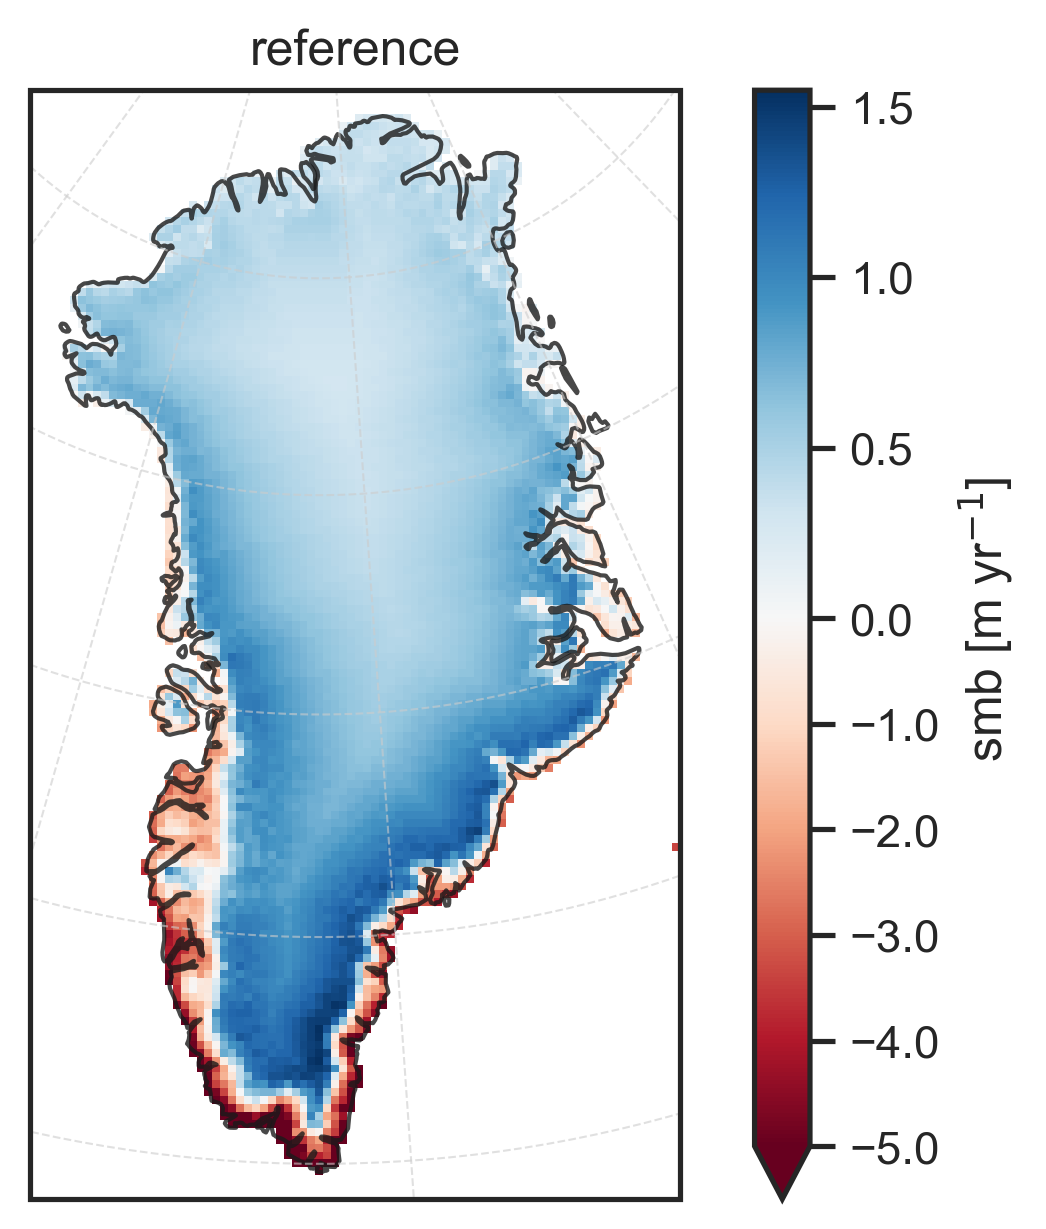
\includegraphics[width=0.45\textwidth]{../../climate-change-scenarios/smb-map-reference.png}
	\caption{SMB calculated from temperature and precipitation fields based on default scaling factors introduced in \cref{tab:smb}; please note that the colorbar uses a different scaling for positive and negative values.}
	\label{fig:smb-ref}
\end{figure}
